 \chapter{Introduction}
 
\pagenumbering{arabic}
\setcounter{page}{1}

Molecular imaging has provided science with great advances during it's history, such as the determination of the helical structure of DNA in 1953~\cite{watson_molecular_1953}, and the discovery of the structure of myoglobin and haemoglobin in 1962~\cite{kendrew_x-ray_1957}.
The \gls{caeis} at the University of Melbourne is an ongoing project that aims to develop a source capable of achieving the `holy grail' of scientific imaging, the \emph{molecular movie}~\cite{dwyer_femtosecond_2006,sciaini_femtosecond_2011}.
A \gls{caeis} also has potential applications with ion beam techniques such \gls{fib} techniques~\cite{mcclelland_bright_2016}, and ion microscopes~\cite{knuffman_cold_2013} as well as use as a particle source for accelerators such as synchrotrons and \glspl{xfel}~\cite{van_oudheusden_electron_2007,zhu_future_2015,mcculloch_cold_2016}.

\section{Making the `Molecular Movie'}

Being able to observe molecular dynamics at an atomic spatial and temporal scale could provide great insight into some of the basic processes of biology and chemistry.
The fabled `molecular movie' refers to capturing the atomic motions of molecular systems as they undergo some transition such as a chemical reaction, protein folding, melting, or even just atomic vibrations.
Molecular movies could provide greater understanding of important biological reactions such as photosynthesis or oxygen transport by haemoglobin.

One of the stepping stones towards molecular movies is single-shot imaging of non-crystalline molecules which would allow structural determination of membrane proteins, an essential step in rational drug design~\cite{hardy_atomic_1987, barrett_discovering_1999, pinto_influenza_1992}.
One of the main techniques in stuctural determination of crystalline targets is electron diffraction which, along with X-ray and neutron methods~\cite{cullity_elements_2001,bacon_x-ray_2013}, has be utilised in structural determination of many materials with atomic resolution.
Continuing research into real-space and diffraction imaging techniques is aiding in the understanding of a growing range of samples as well as providing new types of information on the sample under investigation.

Ultrafast imaging techniques are a relatively recent development and they provide the opportunity to study electronic and atomic dynamics.
Ultrafast techniques also provide an avenue for the imaging of structures that, to date, cannot be imaged by cyrstallographic techniques as some of these techniques should be applicable to uncrystallised samples with imaging being faster than damage processes~\cite{gaffney_imaging_2007,barty_ultrafast_2008,miao_beyond_2015}.
In the past the greatest success with structural determination has been acheived with crystallography which is limited by to samples that can be crystallised.
There are a large number of biological proteins of interest, particularly membrane proteins, that cannot be crystallised and developements in ultrafast imaging techniques is providing a route towards structural determination without crystallisation~\cite{dauter_current_2006,levitt_nature_2009}, cryogenic electron microscopy is also making headway in this area~\cite{henderson_model_1990,zhou_towards_2008}.
Both X-ray and electron imaging techniques are limited by the capabilities of their sources which are undergoing continual developement, in the realms of fundamental physics and engineering.
The techniques using X-rays and electrons each have different advantages and disadvantages with regards to dynamic imaging and structural determination and they often give complementary information.

One proposed method for generating molecular movies involves using a high-brightness ultrashort-duration beam source, such as a \gls{xfel} or future-\gls{caes}, to perform \gls{cdi} on individual molecules~\cite{chapman_femtosecond_2006,dwyer_femtosecond_2006,gaffney_imaging_2007}.
The individual molecules would be dropped one-by-one infront of the illuminating bunches which would be short enough that imaging is completed before damage from the illumination affects the diffraction pattern, see Figure~\ref{figure:molecule_cdi}.
Dynamic processes, such as phase transitions, melting, and pumped vibrational modes, can be studied with this technique if the process can be triggered, say with a precisely timed laser pulse, and by varying the delay between triggering the process and imaging the molecule a `movie' can be constructed.
The random orientation of molecules as they are imaged can be dealt with algorithmically~\cite{yefanov_orientation_2013}.

\begin{figure}
    \center
    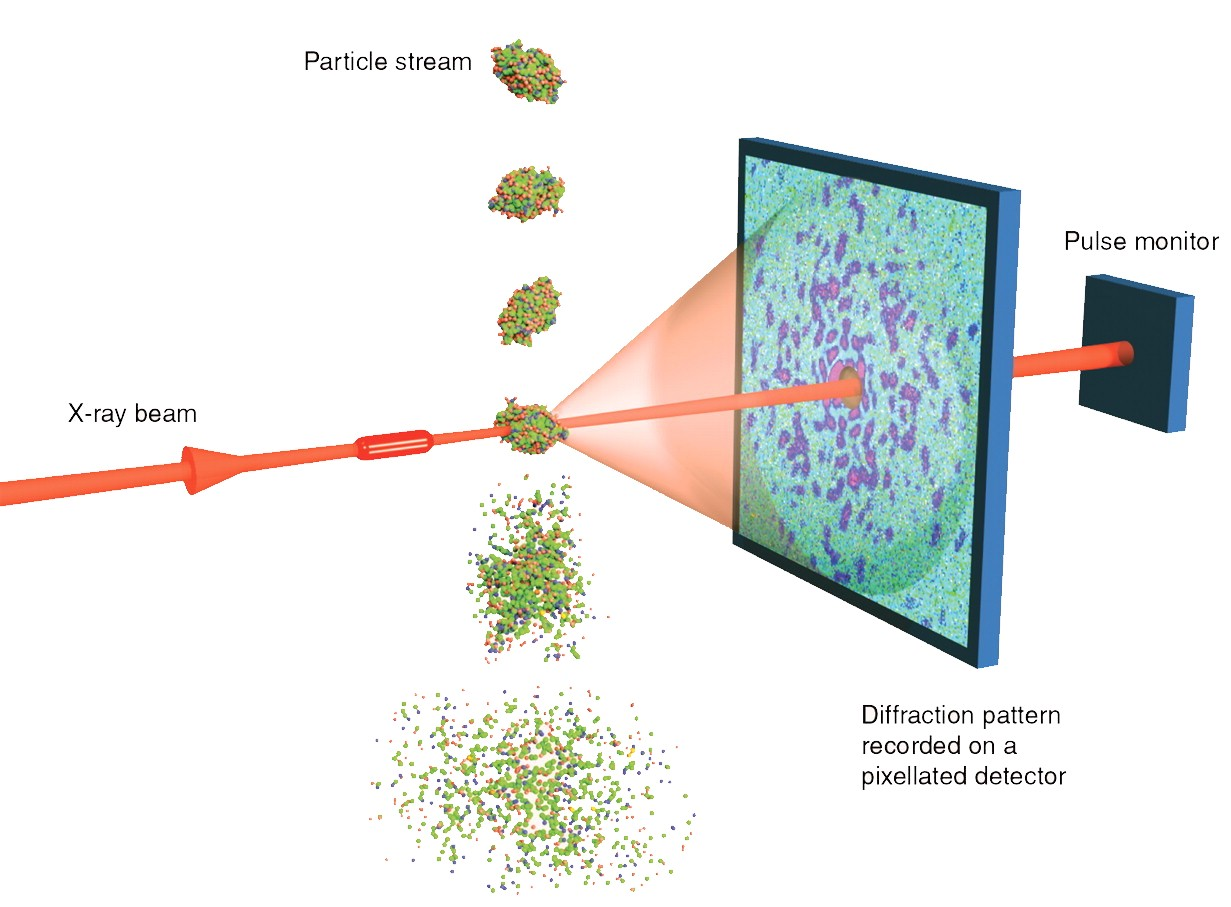
\includegraphics[width=0.65\linewidth]{0intro/Figs/single_molecule_cdi.jpg}
    \caption{Structural determination of single molecules should be possible if a sufficiently bright and short pulse of X-rays is used image the molecule before damage affects the diffraction patter prduced. Electrons could be used in place of X-rays if a suitable source can be developed. Image adapted from Reference~\cite{gaffney_imaging_2007}}
    \label{figure:molecule_cdi}
\end{figure}

Some recent results from X-ray sources are well on the way to producing molecular movies~\cite{pande_femtosecond_2016,nango_three-dimensional_2016}.

\subsection{Ultrafast Coherent Diffractive Imaging}

In order to be able to resolve the structure of single molecules as they are illuminated by the beam there needs to be a sufficient signal such that alignment can be solved and averaging perform, and the imaging need to be complete before the molecule is substantially damaged by the beam~\cite{huldt_diffraction_2003}. Thus a single pulse must be extremely intense and extremely short in duration~\cite{chapman_femtosecond_2006}.
In order to capture dynamics the duration of the pulses must be no larger than the desired temporal resolution and there must be good synchronisation and small jitter between the timing of the imaging pulses and the dynamic processes.

The coherence of the source is also an important consideration for this kind of imaging as the beam must have a coherence length as large as that of the molecule under consideration so that portions of the illuminating wave diffracted from different positions on the molecule interfere coherently.
The diffraction pattern detected is the square of the Fourier coefficients that represents the molecule under examination.
Due to the loss of the complex phase components when the Fourier coefficients are squared it is not possible to direcly invert to recover the structure of the molecules, this is known as the \emph{phase problem}~\cite{rodenburg_phase_1989}.
The most common solution to the phase problem is iterative computational phase-retrieval~\cite{chapman_coherent_2010}.

Ultrafast \gls{cdi} has been demonstrated has been demonstrated previously on micron-scale objects using a \gls{xfel}~\cite{chapman_femtosecond_2006}.

\subsection{Imaging Targets}

Great strides in our understanding of biology and medicine have been made with the knowledge provided by crystallographic techniques over the decades they have been in use.
The structure of biological molecules plays a vital role in their function, with proteins interacting with sub-structures of othr proteins to mediate biological processes, somewhat analogous to a lock and key.
Knowing the structure of biological proteins is essential to fully understanding how the mechanism that protein is involved in function, and can provide vital information to researchers on how to produce drugs to manipulate that mechanism~\cite{aloy_structural_2006,almen_mapping_2009}.
The design and creation of drugs based on knowledge of the structure of the proteins involved in a mchanism is sometimes referred to as \emph{direct drug design} and has had some success to date~\cite{klebe_recent_2000,jhoti_structure-based_2007,mauser_recent_2008}.
The first example of structurally informed direct drug design was the drug dorzolamide which was released to the market in 1995 to reduce intraocular pressure in certain circumstances~\cite{greer_application_1994}.

One of the obvious restrictions on crystallography is that the target sample must be crystallisable in order for it to be imaged and unfortunately there are large numbers of important biological proteins that scientists have been unable to crystallise, notably a large portion of membrane proteins which mediate interactions on the surfaces of cells~\cite{geerlof_impact_2006}.
Alternative structure determination techniques such as ultrafast \gls{cdi} with a \gls{xfel} or \gls{caes} would be able to bypass the crystallisation requirement and thus provide researchers with a wealth of useful information.

The potential to be able to produce molecular movies provides another set of attractive samples.
Knowledge of the changes in molecular structures during many complex and interesting dynamics (such as melting, photosynthesis, molecular phase transitions, or chemical reactions) would prove invalueable to understanding the physics, chemistry and biology of many areas.

\subsection{Ultrafast Imaging}

Damage from high-intensity 

\subsection{Requirements}

Ultra-fast, single-shot, orientation, flux, coherence.

\subsection{X-rays vs. Electrons}



Interaction strength
Wavelength

Current source options

Synchrotrons
XFELs

Photocathode sources
CAESs

\section{Cold-atom electron and ion sources}

The research described by this thesis is part of an ongoing effort to develope an alternative source of electrons and ions that extracts the charged particles from a laser cooled atomic cloud.
Initially the aim of the project was to create ultrafast coherent electron bunches for use in diffraction imaging in a similar way to ultrafast X-ray pulses however it was later realised that \gls{caes} could also serve as an injection source for particle accelerators.
It has also become apparent that by simply reversing the polarity of the accelerator the source can generate high quality ion bunches with similar properties to the electron bunches thus providing a new source for use in ion microscopy and nano-fabrication.

Cold-atom sources operate by carefully ionising atoms in a \gls{mot} such that the resulting ions and electrons are cold and thus the bunches accelerated from those clouds have low emittance and high coherence.
The low transverse temperature of ions and electrons produced by a \gls{caeis} is one of the main advantages of this source however the source also allows for the production ultrafast bunches, arbitrarily shaped bunches and these techniques are applicable to any of the many atomic species that can be laser cooled and trapped.

A \gls{caes} can be thought of as a photocathode electron source with the solid cathode replaced with an ultracold gas which provides the \gls{caes} with a few advantages such as the high quantum efficiency achievable, and near-threshold ionisation producing colder electrons than those from other photocathode sources~\cite{engelen_effective_2014}.
The simplicity of the interactions between photons and atoms allows for the high quantum efficiency to be achieved.
In comparison, in solid cathodes the atoms surrounding a photonic interaction complicate the ionisation and electron extraction processes.
An isolated atom, such as that in the ultracold gas, that interacts with a photon has a much more limited range of potential outcomes, absorption of the photon, radiative decay or ionisation, each with well understood probabilities thus allowing the optimisation of the quantum efficiency~\cite{baranov_field_1994}.

Another advantage of gas photocathodes over solid ones is the lack of optically induced damage from high-intensity laser-fields.
Solid cathodes undergo constant degradation due to the strong fields used and require regular replacement~\cite{dowell_results_1995} whereas the gaseous target in a \gls{caes} is renewed with every bunch produced.

One of the major advantages of \glspl{caeis} is the low temperature of the source which is due to the careful ionisation of the atoms trapped within the \gls{mot}.
The ultracold atoms trapped in the \gls{mot} have temperatures around \unit[100]{$\muup$K} but after ionisation the electrons have temperatures determined by the excess energy from the ionisation process~\cite{engelen_high-coherence_2013,engelen_analytical_2014,sparkes_high-coherence_2014,speirs_identification_2017}.
Precise control over the ionisation is possible due to the well understood physics and high quality lasers available, so it is possible to minimise the excess energy from the ionisation process and electrons produced can have transverse temperature as low as \unit[$\sim$10]{K}~\cite{saliba_spatial_2012}.
Unlike electrons ions produced by the source have their initial temperature determined predominantly by the temperature of the trapped atoms before ionisation, \unit[100]{$\muup$K}, with an ion temperature around \unit[1]{mK}~\cite{debernardi_measurement_2011,murphy_detailed_2014}.

\subsection{Developments}

Arbitrary shaping~\cite{mcculloch_arbitrarily_2011}

Space charge~\cite{murphy_detailed_2014,murphy_increasing_2015,thompson_suppression_2016}

Ionisation~\cite{speirs_identification_2017}

diffraction~\cite{saliba_spatial_2012,speirs_single-shot_2015}


\subsection{Ion Source}

By reversing the polarity of the acceleration stage of beam production in a \gls{caeis} a beam of ions can be produced instead of an electron beam.
Ion beams produced share the same advantages as the electron beams with bunches being shapeable, coherent and low-emittance~\cite{knuffman_cold_2013}.

\Glspl{fib} haves a wide variety of applications such as high-resolution imaging~\cite{scipioni_helium_2008}, sample analysis and nanofabrication~\cite{khizroev_focused-ion-beam-based_2004}.
Liquid metal ion sources are the most commonly used \gls{fib} sources, usually using gallium ions due to it's simplicity and robustness despite gallium having a tendency to contaminate or dstroy various samples.
\Glspl{cais} promise to provide an attractive alternative to conventional sources as they are high brightness, low-emittance and are able to operate with a large range of ions, which could be selected to avoid sample contamination.

\Glspl{cais} have been used to demonstrate microscopy with lithium ions~\cite{knuffman_nanoscale_2011} and chromium ions~\cite{steele_focused_2010} and rubidium ion beams have been characterised and used to demonstrate the suppression of space-charge expansion~\cite{murphy_detailed_2014,thompson_suppression_2016}.

\section{Thesis Outline}

\subsection{Part I}

\subsection{Part II}
